\documentclass[12pt,a4paper]{article}

% 中文支持
\usepackage[UTF8]{ctex}

% 页面设置
\usepackage{geometry}
\geometry{left=2.5cm,right=2.5cm,top=2.5cm,bottom=2.5cm}

% 数学公式
\usepackage{amsmath,amssymb}

% 图片和浮动体
\usepackage{graphicx}
\usepackage{float}
\usepackage{subfigure}

% 表格
\usepackage{array,tabularx,longtable}
\usepackage{booktabs}

% 代码高亮
\usepackage{listings}
\usepackage{xcolor}

% 超链接
\usepackage{hyperref}
\hypersetup{
    colorlinks=true,
    linkcolor=black,
    citecolor=blue,
    urlcolor=blue
}

% 页眉页脚
\usepackage{fancyhdr}
\pagestyle{fancy}
\fancyhf{}
\fancyhead[L]{电子工程训练课程报告}
\fancyhead[R]{\thepage}
\renewcommand{\headrulewidth}{0.4pt}
\setlength{\headheight}{15pt} % fix fancyhdr warning: increase header height

% 代码样式设置
\lstset{
    basicstyle=\ttfamily\small,
    keywordstyle=\color{blue},
    commentstyle=\color{green},
    stringstyle=\color{red},
    numbers=left,
    numberstyle=\tiny\color{gray},
    stepnumber=1,
    numbersep=5pt,
    backgroundcolor=\color{gray!10},
    showspaces=false,
    showstringspaces=false,
    showtabs=false,
    frame=single,
    rulecolor=\color{black},
    tabsize=4,
    breaklines=true,
    breakatwhitespace=false,
    title=\lstname
}

\usepackage{titlesec}
\titleformat{\section}
  {\normalfont\Large\bfseries}
  {\chinese{section}、}
  {0pt}
  {}
% 标题信息
\title{\textbf{电子工程训练课程报告}}
\author{
    \begin{tabular}{ll}
        组号：421-G03
    \end{tabular}
}
\date{}

\begin{document}

% 封面
\maketitle
\thispagestyle{empty}

\newpage
\setcounter{page}{1}


% 正文开始
\section{常用电子仪器的使用}
\subsection{万用表的使用练习}
(1)测量电阻阻值

取三个不同色环的电阻，读取电阻标称值、允许偏差，用万用表测量其阻值并记
录，数据记录如下：
\begin{table}[H]
    \centering
    \begin{tabular}{|c|c|c|c|c|}
        \hline
        电阻编号 & 标称值 (Ω) & 允许偏差 (\%) & 测量值 (Ω) & 偏差 \\ \hline
        R1      & 300k       & ±1            & 292.0k         & 2.7\% \\ \hline
        R2      & 100k       & ±1            & 100.8k        & 0.8\% \\ \hline
        R3      & 10k       & ±2            & 10.50k        & 4.8\% \\ \hline
    \end{tabular}
    \caption{电阻测量数据记录}
    \label{tab:resistance}
\end{table}
观察数据容易发现，偏差相对于允差较大，可能是由于测量时手指触碰电阻引起的，导致测量值不准。

(2)测量电容

取三个不同电容值的电容，读取电容的标称值，用万用表测量其电容并记录，计
算电容偏差。数据记录如下：
\begin{table}[H]
    \centering
    \begin{tabular}{|c|c|c|c|c|}
        \hline
        电容编号 & 标称值 (μF) & 测量值 (μF) & 偏差 \\ \hline
        C1      & 47          & 55.73         & 15.7\% \\ \hline
        C2      & 1           & 1.2001        & 16.7\% \\ \hline
        C3      & 47         & 57.93       & 18.9\% \\ \hline
    \end{tabular}
    \caption{电容测量数据记录}
    \label{tab:capacitance}
\end{table}
偏差集中在15\%到20\%之间，可能是由于电容的标称值本身就有较大误差，或者测量时环境因素影响较大。

(3)测量二极管正向导通电压

取一个二极管，用万用表判断其极性，测量它的正向导通压降，并记录。（将万用
表打到“二极管测量/蜂鸣”档位，按下万用表面板上的“SELECT”按钮，选择“二极管测
量”）。
实验测得二极管的正向导通压降为0.6171V。

(4)利用万用表判断三极管极性

取一个三极管，使用万用表黑表笔接触一极，红表笔分别接触另外两极，如果都可导通，则三极管为pnp结，黑表笔所接触的为基极。如果黑红表笔互换得到类似实验结果，则三极管为npn结，红表笔接触的为基极。
之后用万用表的hFE模式测量三极管放大倍数，可以进一步确定它的集电极和发射极。
如图，本实验使用上述方法，测得所选三极管为npn结，放大倍数为258
\begin{figure}[H]
    \centering
    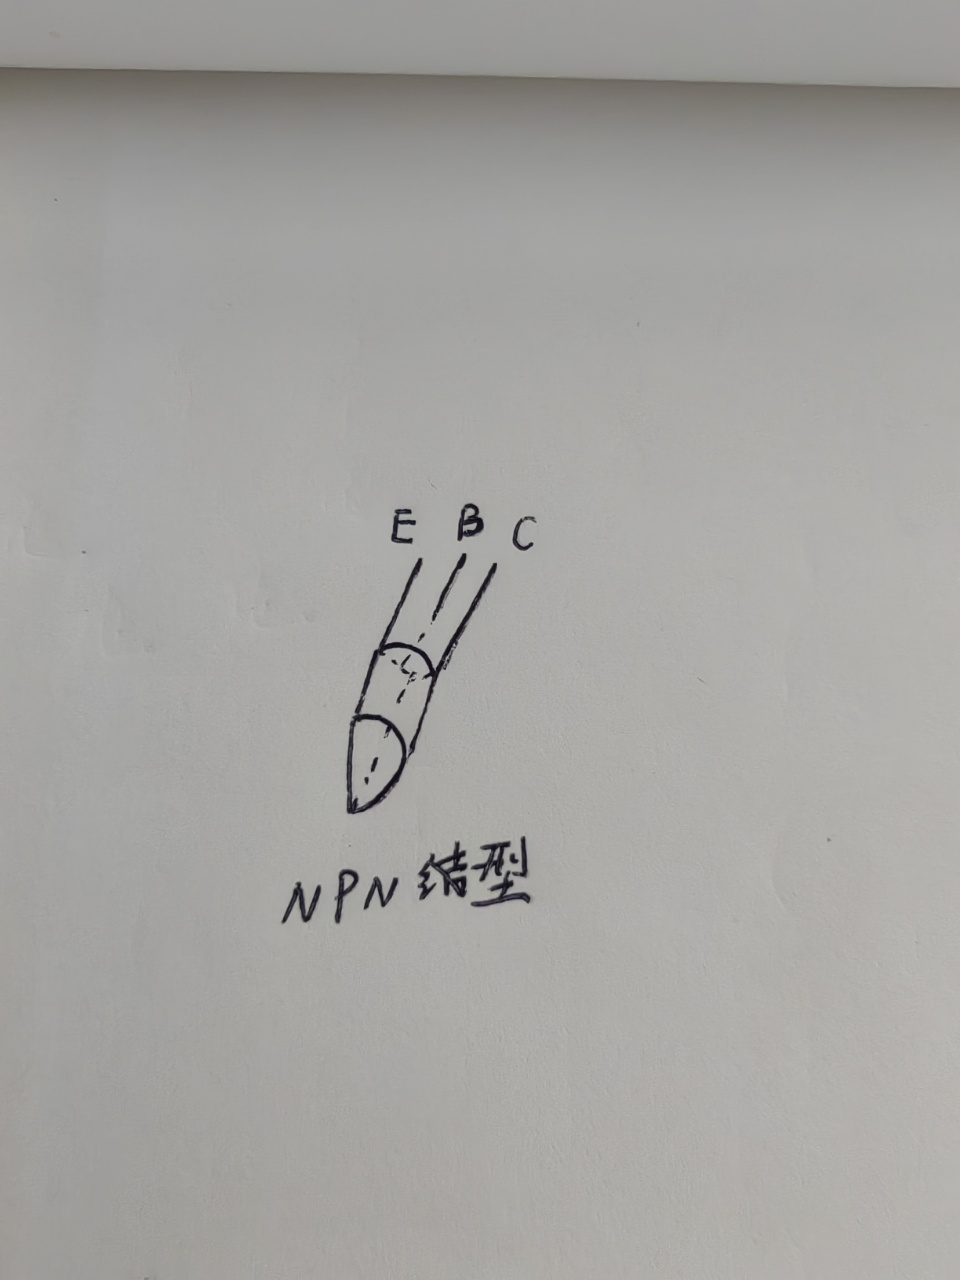
\includegraphics[width=0.4\textwidth]{assets/part1/transistor.jpg}
    \caption{三极管}
    \label{fig:transistor}
\end{figure}
\subsection{电源与万用表使用练习}
(1)设定电源CH1、CH2电压分别为5V、12V，电流均为1A。用万用表直流电压档测量
实际输出电压并记录，计算电压偏差。实验数据如下：
\begin{table}[H]
    \centering
    \begin{tabular}{|c|c|c|c|c|}
        \hline
        通道 & 设定值 (V) & 测量值 (V) & 偏差 \\ \hline
        CH1  & 5          & 5.067       & 1.3\% \\ \hline
        CH2  & 12         & 12.064       & 0.5\% \\ \hline
    \end{tabular}
    \caption{电源输出电压测量数据记录}
    \label{tab:power_supply}
\end{table}
可以看到电压测量值的绝对偏差都在0.06v左右，偏差率在1.5\%以内，说明电源输出电压较为稳定。

(2)设定电源电压分别为正负5V，正负12V，用万用表直流电压档测量并记录实际输出电压，计算电压偏差。实验数据如下：
\begin{table}[H]
    \centering
    \begin{tabular}{|c|c|c|c|c|}
        \hline
        通道 & 设定值 (V) & 测量值 (V) & 偏差 \\ \hline
        +5V  & 5          & 5.028       & 0.6\% \\ \hline
        -5V  & -5         & -5.068      & 1.3\% \\ \hline
        +12V & 12         & 12.067      & 0.6\% \\ \hline
        -12V & -12        & -12.048     & 0.4\% \\ \hline
    \end{tabular}
    \caption{电源串联电压输出测量数据记录}
    \label{tab:power_supply_neg}
\end{table}
可以看到电压测量值的绝对偏差都在0.07v左右，偏差率在1.5\%以内，说明电源在串联情况下输出电压仍较为稳定。

(3)设定电源CH1电压为1V，限定电流为0.5A，用万用表的“2A直流电流”档测量
短路限制电流并记录，计算设置偏差（电流测量时，将红表笔插到左边的2/20A输入孔，测
量结束恢复到电压/电阻测试位置）。实验数据如下：
\begin{table}[H]
    \centering
    \begin{tabular}{|c|c|c|c|c|}
        \hline
        设定值 (A) & 测量值 (A) & 偏差 \\ \hline
        0.5        & 0.4590       & 8.9\% \\ \hline
    \end{tabular}
    \caption{电源短路限制电流测量数据记录}
    \label{tab:short_circuit_current}
\end{table}
设定值与测量值绝对偏差为0.041A，偏差率为8.9\%，说明电源的短路保护功能较为有效。
\subsection{信号源与示波器使用练习}
(1)示波器探头接校准信号源，按傻瓜键“Autoset”，观察记录波形；使用光标法（按
示波器面板上的“Cursor”功能键）读取信号的幅度和周期（或频率）信息，并作相应记录。

信号源选择了正弦波输入，幅值5.00$v_{pp}$，频率1kHz，波形如图。使用光标法读取信号幅值4.99$v_{pp}$，频率1.000kHz，测量值与设定值基本一致。
\begin{figure}[H]
    \centering
    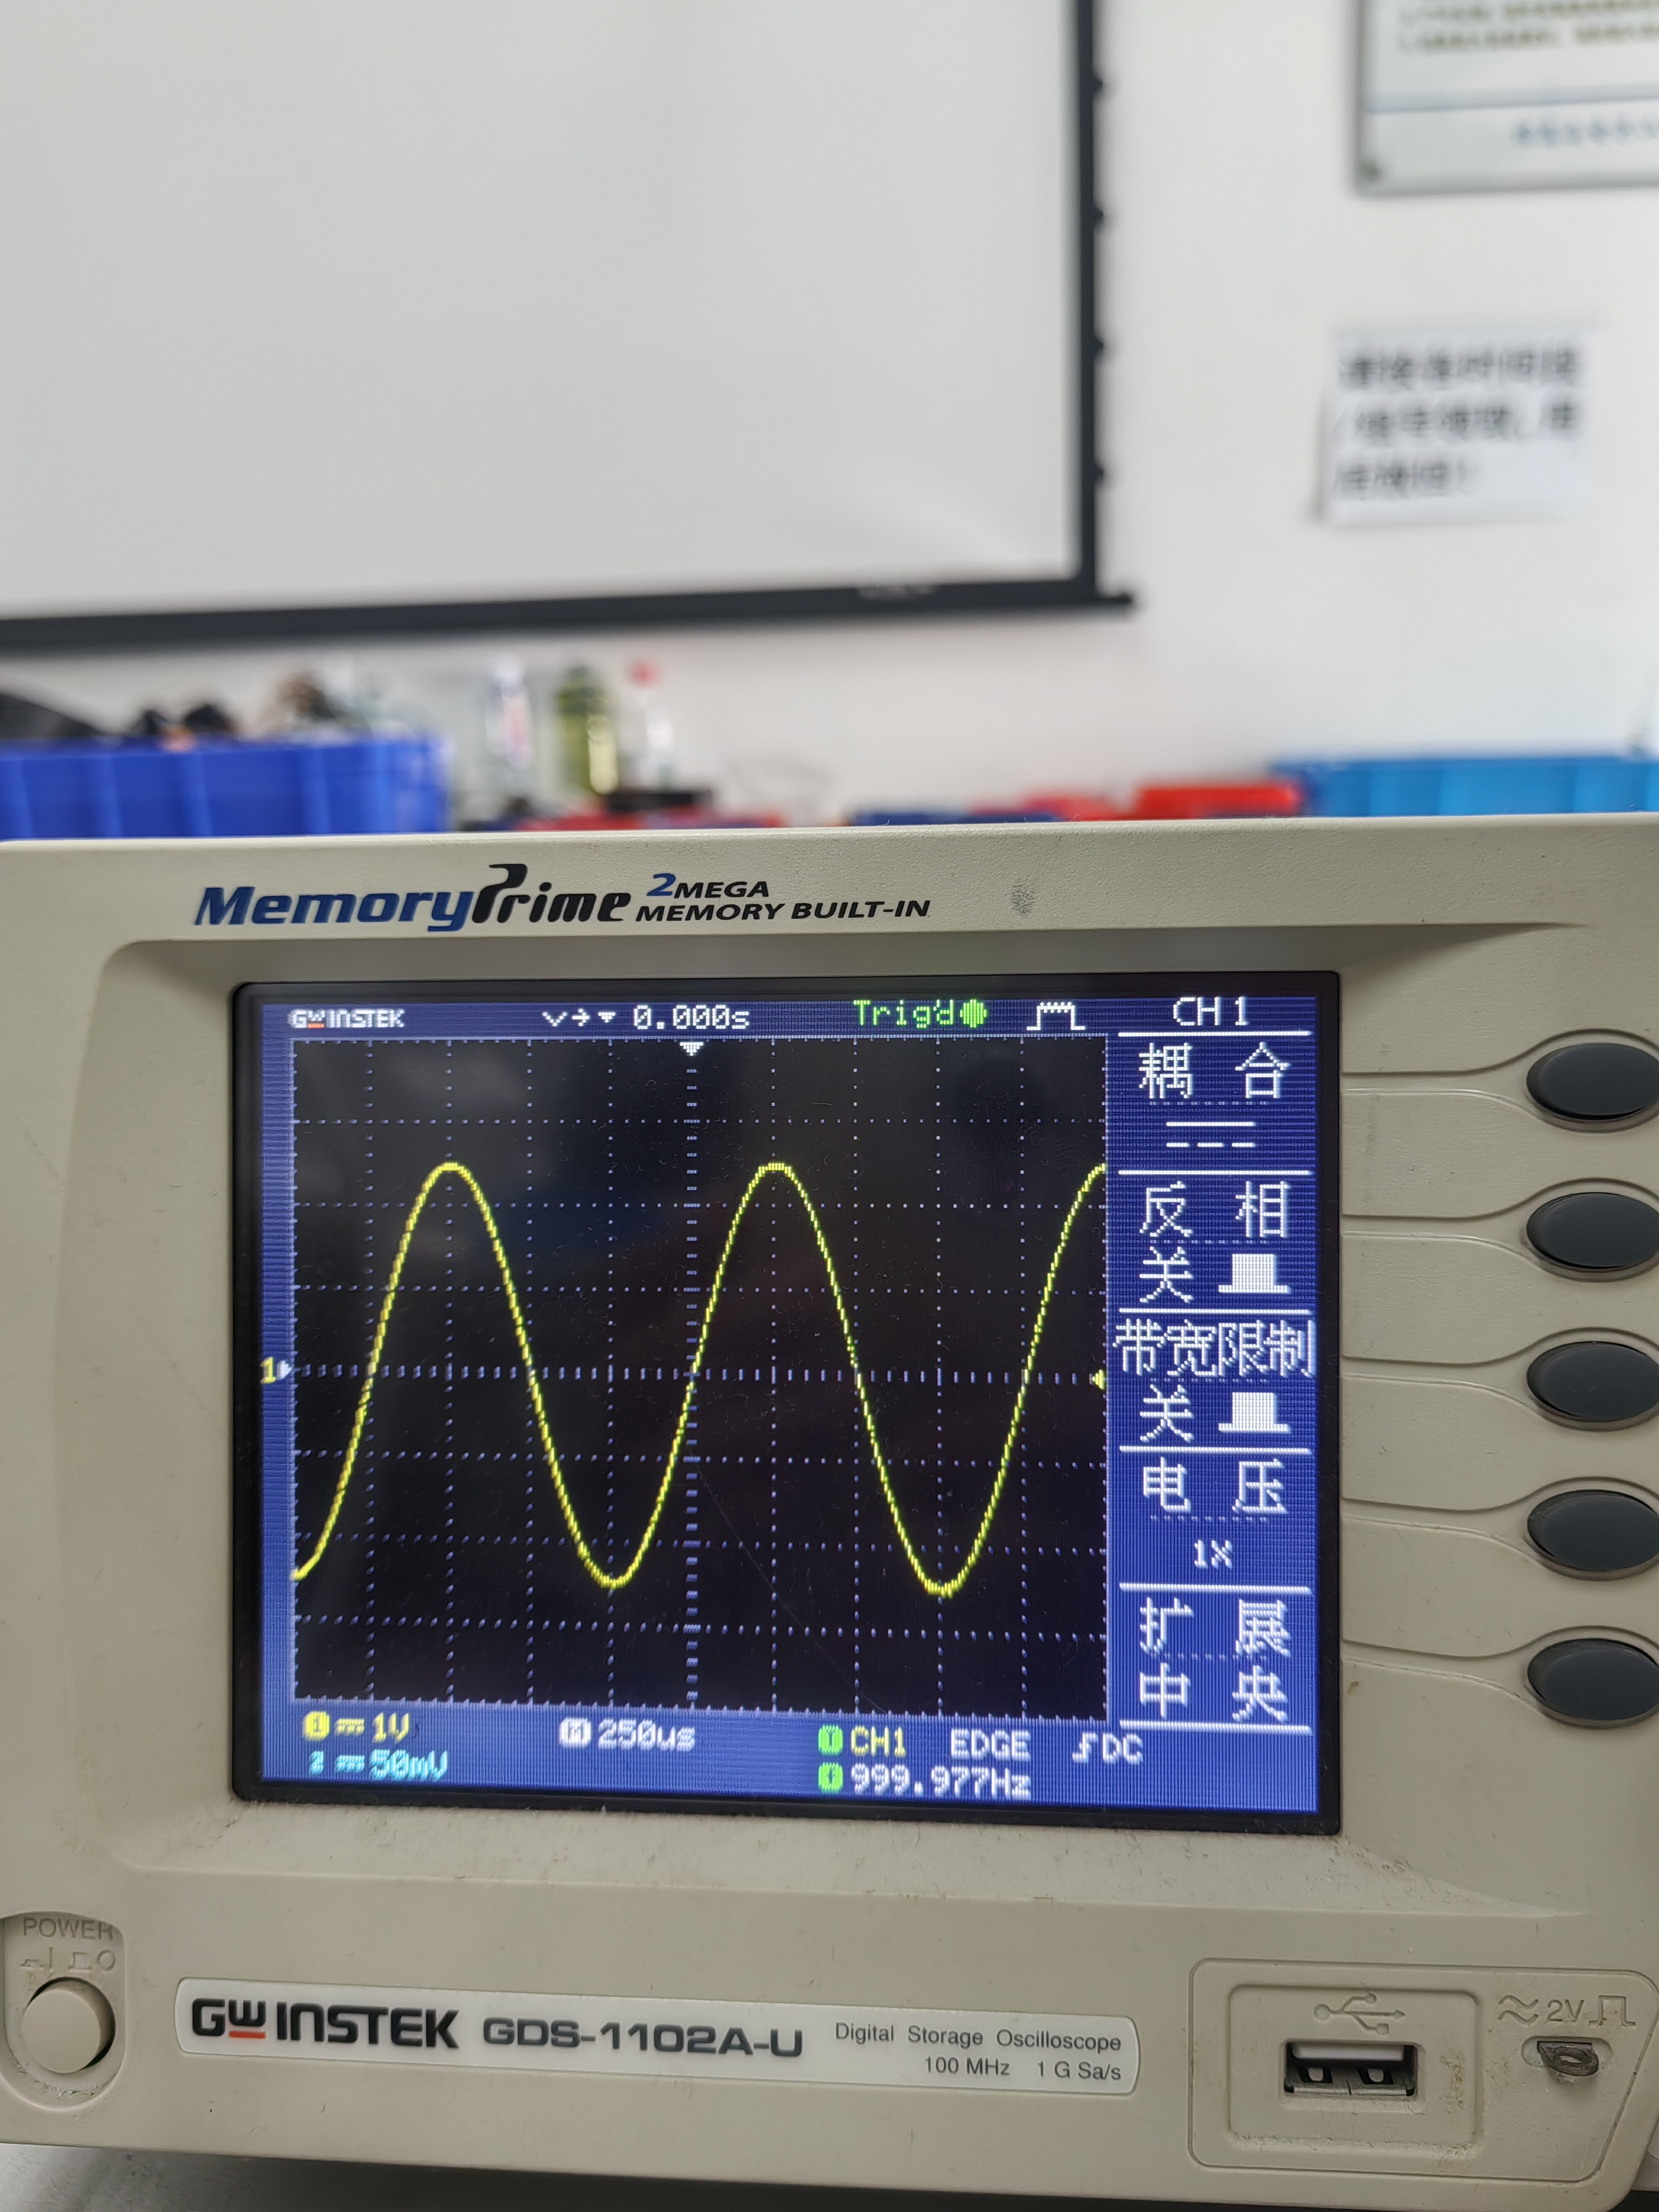
\includegraphics[width=0.6\textwidth]{assets/part1/sine_wave.jpg}
    \caption{示波器显示的正弦波形}
    \label{fig:sine_wave}
\end{figure}
(2)调节信号源，使信号源输出幅度为0.2$v_{pp}$，频率分别为10KHz，100KHz，1MHz，
10MHz 的正弦波信号。用示波器CH1测量信号源的输出，选择触发通道为“CH1”，触发模式
为“自动”，调节触发电平“LEVEL”使得波形能稳定显示。调节相应的量程旋钮“VOLTS/DIV”，
和扫描周期旋钮“TIME/DIV”使得波形显示大小合适，记录设定的电压量程和扫描时间；按
测量键“Measure”，记录测量得到的波形的幅度和时间（或频率）参数。

信号统一为正弦波，幅度0.2$v_{pp}$，频率分别为10KHz，100KHz，1MHz，10MHz。测量数据如下：
\begin{table}[H]
    \centering
    \begin{tabular}{|c|c|c|c|c|}
        \hline
        频率 (Hz) & 电压量程 (mV) & 扫描时间 (/div) & 测量幅度 (mV)  & 测量频率(Hz)  \\ \hline
        10K         & 100                 & 25$\mu s$     & 204     & 12.05K              \\ \hline
        100K        & 100                 & 2.5$\mu s$    & 204     & 122.6K              \\ \hline
        1M      & 100                 & 250ns         & 204     & 1.005M              \\ \hline
        10M      & 100                 & 50ns          & 212     & 9.930M             \\ \hline
    \end{tabular}
    \caption{不同频率正弦波测量数据记录}
    \label{tab:sine_wave_measurements}
\end{table}
可以看到幅度测量值和设定值基本一致，频率测量值也与设定值相符，信号源和示波器均正常工作。

(3)在实验步骤(2)的基础上，改变信号波形：分别为方波、三角波，测量波形的幅
度和时间参数并记录。
信号源输出方波时不支持10MHz频率，其他频率均可输出。幅值仍设定为0.2Vp-p，测量数据如下：
\begin{table}[H]
    \centering
    \begin{tabular}{|c|c|c|c|c|}
        \hline
        频率 (Hz) & 电压量程 (mV) & 扫描时间 (/div) & 测量幅度 (mV)  & 测量频率(Hz)  \\ \hline
        10K         & 50                 & 25$\mu s$     & 218     & 10.00K              \\ \hline
        100K        & 100                 & 2.5$\mu s$    & 216     & 100.0K              \\ \hline
        1M      & 100                 & 250ns         & 228     & 1.000M              \\ \hline
    \end{tabular}
    \caption{不同频率方波测量数据记录}
    \label{tab:square_wave_measurements}
\end{table}

信号源输出三角波时不支持1MHz和10MHz频率，其他频率均可输出。幅值仍设定为0.2Vp-p，测量数据如下：
\begin{table}[H]
    \centering
    \begin{tabular}{|c|c|c|c|c|}
        \hline
        频率 (Hz) & 电压量程 (mV) & 扫描时间 (/div) & 测量幅度 (mV)  & 测量频率(Hz)  \\ \hline
        10K         & 100                 & 25$\mu s$     & 204     & 10.00K              \\ \hline
        100K        & 50                 & 5$\mu s$    & 198     & 100.2K              \\ \hline
    \end{tabular}
    \caption{不同频率三角波测量数据记录}
    \label{tab:triangle_wave_measurements}
\end{table}
可以看到方波、三角波的测量值与设定值基本一致，信号源和示波器均正常工作。

(4)信号源输出信号频率保持200KHz不变，在实验步骤(2)的基础上改变信号的幅
度，在0.5Vp-p与2Vp-p之间变化，步进0.5Vp-p用示波器观察信号的变化，采用光标法分
别测量幅度值并做相应的记录，分别计算测量偏差。

信号源输出频率为200KHz的正弦波，幅值分别设定为0.5Vp-p，1.0Vp-p，1.5Vp-p，2.0Vp-p。测量数据如下：
\begin{table}[H]
    \centering
    \begin{tabular}{|c|c|c|}
        \hline
        设定幅度 (Vp-p)  & 测量幅度 (V)  & 偏差 \\ \hline
        0.5             & 0.520     & 3.8\%              \\ \hline
        1.0             & 0.992   & 0.8\%              \\ \hline
        1.5             & 1.53   & 2.0\%              \\ \hline
        2.0             & 2.00   & 0.0\%              \\ \hline
    \end{tabular}
    \caption{不同幅度正弦波测量数据记录}
    \label{tab:amplitude_variation_measurements}
\end{table}
可以看到幅度偏差均在5\%以内，说明信号源和示波器均正常工作。

\section{电路板调试}
\subsection{呼吸灯调试}
实验操作：

1) 电源调整到 12V，电流 0.5A，连接电源线，打开电源的输出使能。

2) 呼吸灯应该能正常工作，调整呼吸节奏到最快。

3) 示波器测量集成电路 1 脚的波形，示波器采用直流耦合，采用 STOP 使波形停止（频
率太低时触发功能失效），光标法测量波形的幅度（Vp-p），周期。

4) 示波器测量集成电路 7 脚的波形的幅度和周期。

5) 1 脚和 7 脚分别为何种波形？

6) 调整电位器 R3，观察波形周期的变化。

实验数据整理如下：
\begin{table}[H]
    \centering
    \begin{tabular}{|c|c|c|c|}
        \hline
        测量点 & 幅度 (Vp-p) & 周期 (s) & 波形类型 \\ \hline
        集成电路 1 脚 & 4.88V       & 1.270s & 三角波  \\ \hline
        集成电路 7 脚 & 9.43V       & 2.360s & 方波  \\ \hline
    \end{tabular}
    \caption{呼吸灯测量数据记录}
    \label{tab:breathing_light_measurements}
\end{table}
调节电位器R3，两个引脚信号的周期发生变化，在R3旋至逆时针最大程度时周期T=3.160s，顺时针最大程度时周期T=1.380s。可以体会到调节电位器对呼吸灯节奏的影响。
\subsection{幸运转盘调试}
实验操作：

1) 电源调整到电压：5V，电流 0.5A，连接电源线，打开电源的输出使能。

2) 按一下启动键，幸运转盘应该能正常工作。

3) 按住启动键，示波器测量集成电路 U1 的 3 脚波形，示波器采用直流耦合，光标法测
量波形的幅度（Vp-p）、周期和负脉冲宽度。

4) 示波器测量集成电路 U2 的任何一个计数输出脚的波形，记录幅度、周期和正脉冲宽
度，计算占空比。

5) 示波器测量三极管 Q1 发射极电压波形（采用直流耦合），按启动键，发射极电压升
高，灯开始闪烁；松开启动键，电压开始下降，当灯刚好停止闪烁时，记录此时的
发射极（E 极）电压。

实验数据整理如下：
\begin{table}[H]
    \centering
    \begin{tabular}{|c|c|c|c|}
        \hline
        测量点 & 幅度 (Vp-p) & 周期 (s) & 脉冲宽度 (s)   \\ \hline
        集成电路 U1 3 脚 & 3.83V       & 12.40m & 75.00$\mu$s   \\ \hline
        集成电路 U2 计数输出脚 & 1.96V       & 126.0m & 12.80m  \\ \hline
    \end{tabular}
    \caption{幸运转盘测量数据记录}
    \label{tab:luck_wheel_measurements}
\end{table}
可以计算出集成电路U2计数输出脚的占空比为10.16\%。

测量三极管Q1发射极电压，当灯刚好停止闪烁时，发射极电压为2.90V。
\subsection{贴片流水灯调试}

1) 连接电源+3V；

2) 测试 NE555 的输出的信号（3 脚）的幅度和频率；

3) 测量上述信号的上升时间和下降时间；

4) 测试 4017 环形计数器输出波形的周期和脉冲宽度，计算信号的占空比，理论值应该
是多少？

5) 测量 Q1 集电极信号周期。

实验测得NE555输出信号（3脚）的幅度为2.40V，频率为13.33Hz，上升时间为102.0ns，下降时间为104.0ns。

测得4017环形计数器输出波形的周期为740.0ms，脉冲宽度为72.00ms，占空比为9.73\%，理论值为10.0\%。

测得Q1集电极信号周期为730.0ms，与4017输出波形周期比较接近。

\section{实验总结}

：

实验收获

1.熟悉了基本电子仪器的使用方法。包括万用表、电源、信号源和示波器等。为以后电子工程相关实验打下基础。

电源使用需要注意打开电源后仍需要点击输出使能按钮才能输出电压，避免误操作损坏电路。

万用表了解到它除了测量电阻电压电流之外，还可以用于辅助判断二极管极性、三极管极性，测量三极管放大倍数等功能。

示波器使用的难点在于触发设置和波形捕捉，尤其是在低频信号和噪声较大的情况下，如何稳定显示波形是一个挑战。
需要熟悉各种触发模式和耦合方式的使用，以及分度值、波形位置的调整。

2.掌握了电路板的调试流程和技巧。
通过呼吸灯、幸运转盘和贴片流水灯的调试，了解了常见集成电路（如NE555、4017等）的工作原理和应用方法。
学会了使用示波器测量各种信号参数，如幅度、周期、脉冲宽度、占空比等。

调试难点一是信号测量时需要选择合适的耦合方式（直流/交流）和触发模式，确保波形稳定显示。
二是准确判断触点位置，确保测量准确。

3.提高了动手能力和解决实际问题的能力。电路焊接对于我这样的初学者来说是一个挑战，
刚开始焊接的点位不够牢固，焊锡过多或过少都会影响电路的正常工作。通过反复练习和调整，逐渐掌握了焊接技巧。

4.增强了团队合作意识和沟通能力。

课程建议

建议一边讲解一边操作演示，增加实际操作环节，让学生有更多动手实践的机会。同时也避免一次性讲解大量知识，实操时学生遗忘较多的问题。

提高讲解效率，避免拖堂。可以提前准备好实验器材，减少等待时间。

增加课程难度，适当引入一些复杂电路的调试，提升学生的综合能力。



：

1.从焊接方面而言，这段时间我们主要尝试了普通焊接和贴片焊接两种略有差异的焊接思路；
显然贴片焊接作为一种更加规整更加节约空间的焊接方法更符合电路板的实际工作情况，相应的是贴片焊接对操作者的操作精度和稳定性要求的显著提高，
给锡多少和怎样稳定器件都对我这样的初学者提出了不小的挑战；

基于这一点而言，我对课程内容的想法是能否引入更多更为充分的实操机会，弥补并纠正学生在实际焊接时可能出现的疏忽和错漏

2.从电路调试和仪器使用方面而言，我们在基础环节中分别进行了元器件特性测量和实际电路测试。

在基础测量阶段，重点在于熟悉常用电子仪器的基本操作，包括稳流稳压源、万用表、信号发生器与示波器等。
具体内容包括使用万用表测量电阻、电压和电流，辅助判断二极管与三极管的极性，测量三极管的放大倍数，以及掌握示波器的基本使用方法。
由于该部分不涉及实际电路搭建，整体操作难度相对较低。

而进入实际电路调试阶段后，我们借助电路图对NE555等常见集成电路的输入输出特性进行了测量。
调试过程中，首先需注意将电源输出的电压与电流控制在合理范围内，以避免损坏电路元件。
在波形测量环节，主要难点在于如何选取合适的测量基准与触发方式，以获取稳定且易于观察的波形。
此外，峰值点位置的判断偏差和测量时电路触点的抖动也容易引入测量误差。

关于这一部分的教学方式，我建议可以更多采用“边听讲边操作”的形式。目前一次性讲解的内容较多，容易导致部分关键细节被忽略，实践中我们常常需要反复回顾课件内容，影响了学习效率和操作连贯性。

3.最后，在合作方面，我们在实际电路调试过程的不少部分都需要我们组员之间的配合，例如读取引脚输入输出波形时需要两人配合调节读数，这是一项需要充分合作意识和沟通能力的任务，
其反映出的要求也是工程实践中不可或缺的一部分。
\end{document}